% 第9章第2节：对称矩阵特征值的扰动（有序特征值的比较，最小最大原理，谱值区间与正定性保证）。

\section{对称矩阵特征值的扰动}
\label{sec:ls-spectral-sensitivity}
\label{sec:linear-algebra-spectral-stability}
\label{sec:ch06-spectral-stability}
\label{sec:ls-spectral-value-sensitivity}

上一节固定矩阵，只让输入向量带误差。实际中矩阵本身也来自数据：协方差矩阵由有限样本估计，系数矩阵经过测量和舍入。设手中的矩阵与真实矩阵相差$\bm E$，我们只知道误差预算$\lVert\bm E\rVert_2\leq\varepsilon$。由手中矩阵算出的特征值、奇异值、秩和特征子空间，哪些结论对真实矩阵仍然可靠？

谱值的大小、所选子空间的方向、矩阵是否接近秩亏，是不同的输出，各自需要相应的界与条件。本节和随后五节按对象分开讨论：先是对称矩阵的特征值与特征子空间，再是一般方阵的特征值与特征子空间，最后是任意矩阵的奇异值与奇异子空间。对称矩阵的结论最完整，后面几节或者借助它，或者说明缺少对称结构时结论怎样变弱。

本节的界都是有限变化界，对任意大小的$\bm E$成立，不需要微分。在可微条件下求所选特征值分支沿指定方向的一阶响应，留给第~\ref{chap:differential-perturbation-analysis}章（第~\ref{sec:multivariable-eigenvalue-differential}节与第~\ref{sec:multivariable-eigenvector-differential}节）。

本节取实对称矩阵$\bm S\in\mathbb R^{d\times d}$与对称扰动$\bm E$。二者的特征值都是实数，记$\bm S$的特征值为$\lambda_1(\bm S)\geq\cdots\geq\lambda_d(\bm S)$，$\bm S+\bm E$的特征值也按降序记为$\lambda_k(\bm S+\bm E)$，再按同一次序逐个比较，把$\lambda_k(\bm S)$看作$\lambda_k(\bm S+\bm E)$的估计。目标是为每个特征值给出区间，并据此判断正负性和正定性。

图~\ref{fig:ls-perturbation-ellipse}画出一个正定矩阵（图中记为$\bm A$）受扰动前后的二次型椭圆：半轴长微变，主轴微转。半轴长对应特征值，主轴对应特征方向；本节先处理前者，主轴的转动留到第~\ref{sec:ls-subspace-sensitivity}节。

\begin{figure}[htbp]
 \centering
 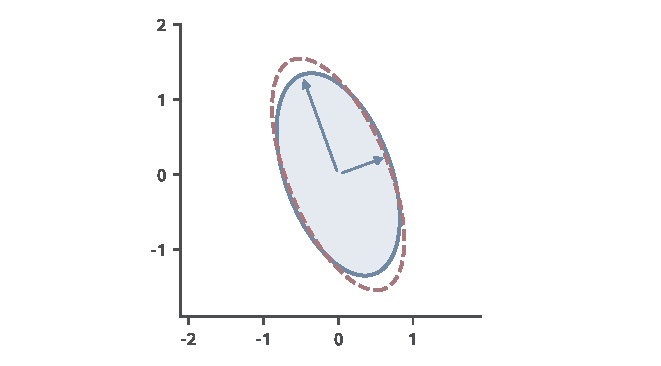
\includegraphics[width=112mm]{figures/00-shared/mathematical-preliminaries-upper/02-linear-spaces/matplotlib/ls-perturbation-ellipse/ls-perturbation-ellipse.pdf}
 \caption{对称矩阵微扰的谱与方向。实线椭圆$\bm x^\top\bm A\bm x=1$对应$\bm A$（特征值$2$与$0.5$，主轴
 方向$20^\circ$），虚线对应$\bm A+\bm E$（$\lVert\bm E\rVert_2\approx0.193$）：轴
 微旋、半轴微变。新特征值约$2.18$与$0.37$，偏移$0.18$、$0.13$均小于
 $\lVert\bm E\rVert_2$，符合Weyl界；未扰动的谱隙$\delta=\lambda_1-\lambda_2=1.5$越大，
 特征方向越不易被微扰转动。}
 \label{fig:ls-perturbation-ellipse}
\end{figure}

\subsection{有序特征值的比较}

扰动对同一方向上二次型的影响很容易估计：由Cauchy--Schwarz不等式，对任意$\bm x$，
\[
 |\bm x^\top\bm E\bm x|\leq\lVert\bm x\rVert_2\lVert\bm E\bm x\rVert_2\leq\lVert\bm E\rVert_2\lVert\bm x\rVert_2^2 .
\]
所以$\bm S$与$\bm S+\bm E$在同一个单位向量上的二次型值相差不超过$\lVert\bm E\rVert_2$。难点在于把这个逐方向的比较传到第$k$个特征值上：两个矩阵的特征方向一般不同，不能直接拿同一个特征向量比较。

办法是用子空间刻画有序特征值。由谱分解，第$k$个特征值把前$k$个特征方向与后$d-k+1$个特征方向分开，二次型在这两组方向张成的子空间上分别不小于、不大于$\lambda_k$。

\begin{lemma}[特征子空间上的二次型界]
\label{lem:ls-eigen-subspace-quadratic-bounds}
\label{lem:ls-restricted-rayleigh}
设$\bm S\in\mathbb R^{d\times d}$实对称，特征值为$\lambda_1\geq\cdots\geq\lambda_d$，对应的标准正交特征向量为$\bm q_1,\ldots,\bm q_d$。对$1\leq k\leq d$，记$\mathcal V_k=\operatorname{span}\{\bm q_1,\ldots,\bm q_k\}$，$\mathcal W_k=\operatorname{span}\{\bm q_k,\ldots,\bm q_d\}$。则
\[
 \bm x^\top\bm S\bm x\geq\lambda_k\lVert\bm x\rVert_2^2\quad(\bm x\in\mathcal V_k),\qquad
 \bm x^\top\bm S\bm x\leq\lambda_k\lVert\bm x\rVert_2^2\quad(\bm x\in\mathcal W_k),
\]
两式在$\bm x=\bm q_k$时都取等号。
\end{lemma}
\begin{proof}
对$\bm x=\sum_{i\leq k}c_i\bm q_i\in\mathcal V_k$，由二次型展开式~\eqref{eq:matrix-analysis-quadratic-spectral-form}，$\bm x^\top\bm S\bm x=\sum_{i\leq k}\lambda_ic_i^2\geq\lambda_k\sum_{i\leq k}c_i^2=\lambda_k\lVert\bm x\rVert_2^2$，因为$i\leq k$时$\lambda_i\geq\lambda_k$。对$\mathcal W_k$中的向量同理，只是$i\geq k$时$\lambda_i\leq\lambda_k$。取$\bm x=\bm q_k$时只有一项，两式都成为等式。
\end{proof}

两个子空间的维数分别是$k$与$d-k+1$，和为$d+1$，超过了空间的维数。由维数公式，任一$k$维子空间与任一$d-k+1$维子空间的交至少是一维的：
\[
 \dim(\mathcal V\cap\mathcal W)\geq\dim\mathcal V+\dim\mathcal W-d=1 .
\]
这样就能在两个矩阵各自的特征子空间中找到一个公共方向，在这个方向上比较二次型。

\begin{theorem}[Weyl特征值扰动界]
\label{thm:ls-weyl-eigenvalue}
设$\bm S,\bm E\in\mathbb R^{d\times d}$实对称。对每个$k=1,\ldots,d$，按降序配对的特征值满足
\begin{equation}
 |\lambda_k(\bm S+\bm E)-\lambda_k(\bm S)|\leq\lVert\bm E\rVert_2 .
 \label{eq:matrix-analysis-weyl-eigenvalue-perturbation}
\end{equation}
\end{theorem}
\begin{proof}
记$\widetilde{\bm S}=\bm S+\bm E$，$c=\lVert\bm E\rVert_2$。取$\bm S$前$k$个特征向量张成的$\mathcal V_k$，以及$\widetilde{\bm S}$第$k$个到第$d$个特征向量张成的$\widetilde{\mathcal W}_k$。由维数公式，二者有公共的单位向量$\bm x$。对$\bm S$与$\widetilde{\bm S}$分别使用引理~\ref{lem:ls-eigen-subspace-quadratic-bounds}，得
\[
 \lambda_k(\bm S)\leq\bm x^\top\bm S\bm x,\qquad
 \bm x^\top\widetilde{\bm S}\bm x\leq\lambda_k(\widetilde{\bm S}).
\]
又$\bm x^\top\widetilde{\bm S}\bm x=\bm x^\top\bm S\bm x+\bm x^\top\bm E\bm x\geq\bm x^\top\bm S\bm x-c$，三式连起来，
\[
 \lambda_k(\widetilde{\bm S})\geq\bm x^\top\widetilde{\bm S}\bm x\geq\bm x^\top\bm S\bm x-c\geq\lambda_k(\bm S)-c .
\]
交换两个矩阵的角色，把$\bm S=\widetilde{\bm S}+(-\bm E)$看作$\widetilde{\bm S}$的扰动，而$\lVert-\bm E\rVert_2=c$，同样得到$\lambda_k(\bm S)\geq\lambda_k(\widetilde{\bm S})-c$。两式合起来即为结论。
\end{proof}

证明只用了谱分解、维数公式和同一方向上二次型的比较，没有求任何二次型的最大值或最小值。它也不要求特征值彼此分开：重特征值时，$\bm q_k$可以在特征空间中任意选取，引理与证明都不受影响。

\subsection{最小最大原理}

证明中的论证还给出单个有序特征值的一种不依赖特征向量的刻画。把公共方向的论证用于任意子空间，就得到下面的结论。

\begin{theorem}[Courant--Fischer]
\label{thm:matrix-analysis-courant-fischer}
\label{eq:matrix-analysis-courant-fischer}
设$\bm S\in\mathbb R^{d\times d}$实对称，特征值为$\lambda_1\geq\cdots\geq\lambda_d$。对$k=1,\ldots,d$，
\begin{equation*}
\begin{aligned}
 \lambda_k
 &=\max_{\dim\mathcal V=k}\ \min_{\bm x\in\mathcal V,\lVert\bm x\rVert_2=1}\bm x^\top\bm S\bm x\\
 &=\min_{\dim\mathcal W=d-k+1}\ \max_{\bm x\in\mathcal W,\lVert\bm x\rVert_2=1}\bm x^\top\bm S\bm x .
\end{aligned}
\end{equation*}
\end{theorem}
\begin{proof}
先说明内层的最小值与最大值取得到。设$\mathcal V$是$k$维子空间，$\bm U\in\mathbb R^{d\times k}$的列是它的标准正交基。$\bm x=\bm U\bm y$是$\mathcal V$中的单位向量，当且仅当$\bm y$是$\mathbb R^k$中的单位向量，且$\bm x^\top\bm S\bm x=\bm y^\top\bm M\bm y$，其中$\bm M=\bm U^\top\bm S\bm U$是$k$阶实对称矩阵。对$\bm M$用谱定理与二次型展开式，单位向量上的$\bm y^\top\bm M\bm y$是$\bm M$的特征值的加权平均，最小值与最大值分别是$\bm M$的最小、最大特征值，并在相应的特征向量处取到。

再证第一式。由引理~\ref{lem:ls-eigen-subspace-quadratic-bounds}，$\mathcal V_k$中单位向量的二次型不小于$\lambda_k$，且在$\bm q_k$处等于$\lambda_k$，所以外层的最大值至少为$\lambda_k$。反过来，任一$k$维子空间$\mathcal V$与$\mathcal W_k$有公共的单位向量$\bm x$，它的二次型不超过$\lambda_k$，所以$\mathcal V$上的最小值不超过$\lambda_k$。两方面合起来，外层最大值等于$\lambda_k$，并在$\mathcal V_k$处取到。

第二式交换两组特征向量的角色：$\mathcal W_k$上单位向量的二次型的最大值恰为$\lambda_k$；任一$d-k+1$维子空间$\mathcal W$与$\mathcal V_k$有公共的单位向量，其二次型不小于$\lambda_k$，所以$\mathcal W$上的最大值不小于$\lambda_k$。
\end{proof}

这一定理称为\term{最小最大原理}（min-max principle）。它只涉及子空间与二次型，不要求先知道特征向量；Weyl界也可以由它推出，只需对同一个子空间比较$\bm S$与$\bm S+\bm E$的二次型。$k=1$与$k=d$时，内层只剩一个子空间，结论化为二次型在单位球面上的最大值与最小值；第~\ref{chap:matrix-approximation}章把$\bm x^\top\bm S\bm x/\bm x^\top\bm x$称为Rayleigh商，并从选择最优方向的问题出发研究这两个极值。那里的迹极值汇总$k$个正交方向的贡献，刻画前$k$个特征值之和；最小最大原理刻画的是单个有序特征值。

\subsection{谱值区间与正定性保证}

由Weyl界，若$\lVert\bm E\rVert_2\leq\varepsilon$，每个真实特征值都落在区间$[\lambda_k(\bm S)-\varepsilon,\lambda_k(\bm S)+\varepsilon]$内。这个绝对误差界不要求特征值彼此分开，单重与重复特征值都适用。但它是绝对误差界：特征值本身接近零时，区间宽度$2\varepsilon$可能与特征值同量级，不能据此宣称相对误差也小。

区间立刻给出特征值符号的判断。若区间不含零，符号由区间确定；若区间含零，当前的误差预算不足以判断符号。例如$\bm S=\operatorname{diag}(1,\varepsilon/2)$，$0<\varepsilon<1$：取$\bm E=\bm0$时第二个特征值为正，取$\bm E=-\varepsilon\bm e_2\bm e_2^\top$时它变为$-\varepsilon/2$，两种扰动都满足预算。正定矩阵沿一条线段变化时，还可以得到对整条线段一致的下界。
\begin{theorem}[特征值的符号与正定性保持]
\label{thm:ls-eigenvalue-sign-definiteness}
设$\bm S,\bm E\in\mathbb R^{d\times d}$实对称，$\lVert\bm E\rVert_2\leq\varepsilon$。
\begin{enumerate}
 \item 若$\lambda_k(\bm S)>\varepsilon$，则$\lambda_k(\bm S+\bm E)>0$；若$\lambda_k(\bm S)<-\varepsilon$，则$\lambda_k(\bm S+\bm E)<0$。
 \item 若$\bm S$正定且$\varepsilon<\lambda_{\min}(\bm S)$，则对一切$t\in[0,1]$，
 \[
  \lambda_{\min}(\bm S+t\bm E)\geq\lambda_{\min}(\bm S)-\varepsilon>0 ,
 \]
 从而线段$\{\bm S+t\bm E:0\leq t\leq1\}$上的矩阵都正定。
\end{enumerate}
\end{theorem}
\begin{proof}
第1条：由定理~\ref{thm:ls-weyl-eigenvalue}，$\lambda_k(\bm S+\bm E)\geq\lambda_k(\bm S)-\varepsilon>0$；负号情形同理，$\lambda_k(\bm S+\bm E)\leq\lambda_k(\bm S)+\varepsilon<0$。第2条：对$t\in[0,1]$，$t\bm E$对称且$\lVert t\bm E\rVert_2=t\lVert\bm E\rVert_2\leq\varepsilon$。对最小特征值$\lambda_d$应用定理~\ref{thm:ls-weyl-eigenvalue}，得$\lambda_{\min}(\bm S+t\bm E)\geq\lambda_{\min}(\bm S)-\varepsilon>0$。实对称矩阵的特征值全为正时，由二次型展开式~\eqref{eq:matrix-analysis-quadratic-spectral-form}，它是正定的。
\end{proof}
第2条的下界$\lambda_{\min}(\bm S)-\varepsilon$与$t$无关。后文对正定矩阵求逆、开方或取对数时，常需确认整条线段都留在这些运算的定义域内，并且离定义域边界有一致的距离，例如第~\ref{sec:multivariable-logdet-perturbation}节估计对数行列式的变化；这个下界正好提供这一保证。

最后用一个例子检查界的精确程度，并看到有限变化界与可微性是两回事。
\begin{example}[重根处的最大特征值]
\label{ex:ls-weyl-double-root}
取$\bm S(t)=\operatorname{diag}(t,-t)$，$t\in\mathbb R$，从重根$\bm S(0)=\bm0$出发看最大特征值怎样移动。$\bm S(0)$的特征值$0$是二重根；$t\neq0$时两个特征值$\pm t$分开，排序后的最大特征值为$|t|$。

它相对于$\bm S(0)$的变化是$|t|$，恰好等于$\lVert\bm S(t)-\bm S(0)\rVert_2=|t|$，所以界~\eqref{eq:matrix-analysis-weyl-eigenvalue-perturbation}在这里取等号，不能再改进；同时也说明重根并不妨碍有限的绝对误差界。但有界的变化不等于光滑的变化：$|t|$在$t=0$处左导数为$-1$、右导数为$1$，排序后的最大特征值在重根处没有双侧导数。原因是$t$变号时，最大特征值从$t$这一支换到$-t$那一支。
\end{example}
第~\ref{sec:multivariable-local-condition-number}节再用这个例子区分有限敏感性与可微性；第~\ref{sec:multivariable-eigenvalue-differential}节在特征值简单的条件下，另行研究所选分支的一阶响应。
